\documentclass{article}
\usepackage[utf8]{inputenc}
\usepackage{amssymb}
\usepackage{tikz}
\usepackage{amsmath}
\usepackage{relsize}
\usepackage{mathtools}
\usepackage{textcomp}
\usepackage{eurosym}
\usepackage{amssymb}
\usepackage{systeme}
\usepackage{mathtools}
\usepackage{todonotes}
\title{Results}
\author{Roman Oort}
\date{\today}

%%% PERSONAL SHORTCUTS
\DeclareMathOperator*{\plim}{plim}
\newcommand{\T}{\textbf{T}}
\newcommand{\Tij}{\textbf{T}_{ij}}
\newcommand{\Soc}{(\T(n))^{\infty}_{n=1}}
\newcommand{\beli}[3][2]{p_{#2}^{(#3)}}
\newcommand{\belvec}[2]{\textbf{p}^{(#2)}}

\begin{document}

\maketitle

\tableofcontents
\newpage
\section{Results}

All results obtained and discussed in the following section are generated with an identical network structure, unless mentioned otherwise. The networks used are all directed networks, with an increased degree, using the default distribution for the degree increase. Furthermore, the probability of a self-link is $1$, meaning that every agent will have a link to itself. Finally, uniform weight initialization was applied. Furthermore, whenever an updating rule did not lead to uniform convergence, the mean of the belief vector was taken as the convergent belief.

\newpage

\subsection{Cooperative Networks}

As can be seen in Figure \ref{coop:compare}, in a cooperative network all updating rule behave quite similar. The convergent belief differs the most for smaller network. However, as the network size increases this difference dissipates, and the convergent beliefs become more and more similar, both to the other updating rules \emph{and} the assumed truth of the model.

\noindent However, while the convergent beliefs are mostly similar, the standard deviation of the convergent belief vector does differ significantly between updating rules. Where the regular and thresholded DeGroot mechanics have no deviation in the convergent belief vector, meaning they have a uniform convergent belief held by every agent, the other updating rules end up with a non-insignificant amount of variation in the belief vector. This means that, at the time of convergence, it is not the case that the different agents all hold the same beliefs, but rather, while their opinions may not change anymore, they still hold different opinions. 

\noindent Finally, the thresholded and regular DeGroot mechanics both reach convergence in the same amount of time, while the other updating rules are significantly faster to reach the point of convergence.

\begin{center}
    \begin{figure}[!htbp]
        \centering
        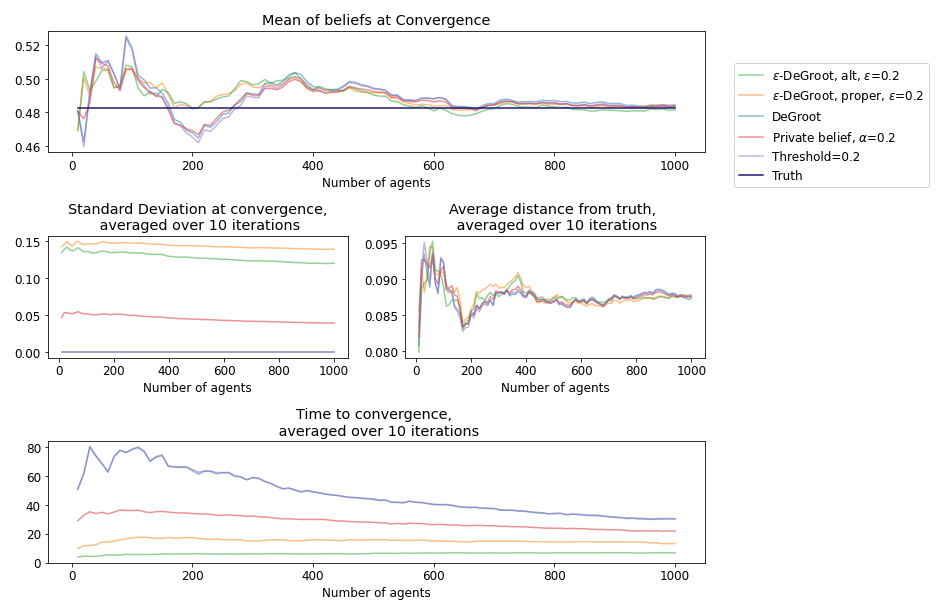
\includegraphics[width=1.2\textwidth]{ThesisKI/Images/WisdomCompare0.png}
        \caption{Convergence Behaviour Threshold Updating}
        \label{coop:compare}
    \end{figure}
\end{center}

\newpage

\subsection{Non-cooperative networks, $n=1$}

Where the different updating rules behaved in a similar fashion as the regular DeGroot updating mechanics in a fully cooperative network, significant differences occur when applied to a network with even one non-cooperative agent, as demonstrated in Figure \ref{noncoop1:compare}. 

\noindent First of all, as expected, under regular DeGroot dynamics the convergent opinion becomes that of the non-cooperative agent, and the same goes for the thresholded DeGroot mechanics. Furthermore, again as expected, this belief is held by every agent in the network, which is expressed by the $0$ standard deviation of the convergent belief vector of these updating rules. However, the other three updating mechanics exhibit vastly different behaviour. Instead of converging towards the opinion of the non-cooperative agent, the network still converges towards the truth. However, once again, this is not a uniform convergence, as there still is some standard deviation in the convergent belief vector, though this appears to decline ever so slightly as the network size increases.

\noindent Finally, the updating time for both the regular and the thresholded DeGroot mechanics behave nearly identical, and both display a significant increase in convergence time, whereas the other three updating rules do not appear to show significantly slower convergence. This increase in convergence time can be explained by the presence of the single non-cooperative agent, whose influence has to spread throughout the entire network, taking more and more time to reach every agent as the network size increases. Furthermore, this appears to be a non-factor for the other updating rules, where the non-cooperative agent is not nearly as formative, or even at all, for the convergent opinion, making it so that it will not significantly impact the convergence time as a result.

\begin{center}
    \begin{figure}[!htbp]
        \centering
        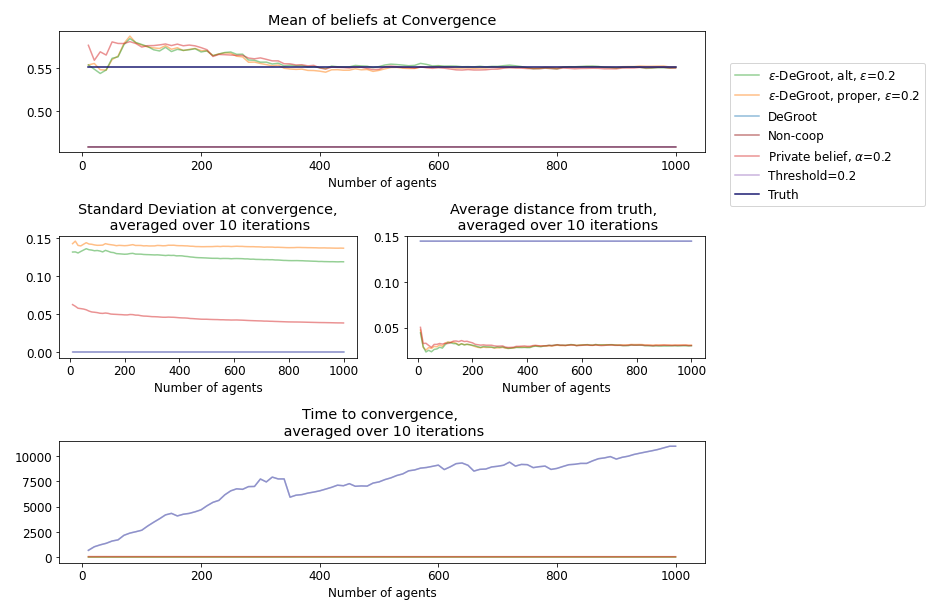
\includegraphics[width=1.2\textwidth]{ThesisKI/Images/WisdomCompare1.png}
        \caption{Convergence Behaviour Threshold Updating}
        \label{noncoop1:compare}
    \end{figure}
\end{center}

\subsection{Non-cooperative networks, $n > 1$}

\end{document}